\documentclass{beamer}
\graphicspath{{./figures/}} 
\mode<presentation>
{
  \usetheme{default} 
  \usecolortheme{default}
  \usefonttheme{default}
  \setbeamertemplate{navigation symbols}{}
  \setbeamertemplate{caption}[numbered]
} 

\usepackage[portuguese]{babel}
\usepackage[utf8]{inputenc}
\usepackage{graphicx}

\title[]{Pesquisa de Algoritmo Estocástico para o Problema U-Curve}
\author{Gustavo Estrela}
\institute{Universidade de São Paulo e Texas A\&M University}
\date{\today}

\begin{document}

\begin{frame}
  \titlepage
\end{frame}

\section{Objetivo}
\begin{frame}{Objetivo}
\begin{itemize}
  \item Estudo do algoritmo IUBB.
      \vskip 5em
  \item Implementação de uma variante estocástica do IUBB.
\end{itemize}
\end{frame}

\section{O Algoritmo IUBB}
\begin{frame}{O Algoritmo IUBB}
    \begin{itemize}
        \item{Baseado no UBB.}
        \vskip 5em
        \item{Duas ideias principais:}
        \begin{itemize}
            \vskip 1em
            \item{Atualização iterativa de cadeias ótimas.}
            \vskip 1em
            \item{Uso da bisecção na procura do mínimo de uma cadeia.}
        \end{itemize}
    \end{itemize}
\end{frame}

\section{Introdução do erro}
\begin{frame}{Introdução do erro}
    \begin{itemize}
        \item{Assumimos erro com distribuição normal com média zero e
            variância $\sigma^2$.}
        \item{Efeitos do erro no algoritmo IUBB.}
        \begin{figure}[h]
            \includegraphics[page=15, clip, trim=12cm 10.7cm 3cm 12cm,
                scale=.8]{IUBB_submit}
            \caption{Efeito de um erro senoidal nos algoritmos UBB e 
        IUBB \protect\cite{iubb}}
        \end{figure}
    \end{itemize}
\end{frame}

\section{Algoritmo de Bisecção Mid-neighbour}
\begin{frame}{Algoritmo de Bisecção Mid-neighbour}
    \begin{itemize}
        \item{Não usa informação sobre o erro.}
        \item{Ideia de restringir o espaço de busca como uma 
            bisecção.}
        \item{Conceito de confiança sobre a diferença observada entre
            elementos avaliados.}
        \item{Decide em qual porção do espaço de busca o mínimo está
            baseado nas diferenças entre os elementos que estão no meio
            da cadeia, no meio da primeira metade da cadeia e no meio da 
            segunda metade da cadeia.}
        \item{Quando a confiança não é "suficiente", divide-se a cadeia
            em dois pedaços e resolve-se o problema em ambas partes.}
    \end{itemize}
\end{frame}

\section{Algoritmo Estocástico I}
\begin{frame}{Algoritmo Estocástico I}
    \begin{itemize}
        \item{Mantém uma função massa de probabilidade $f$ que diz a
            probabilidade de um elemento da cadeia ser o elemento de
            custo mínimo.}
        \item{A cada iteração, avaliam-se $x$, $y$ e $z$ tal que 
            $F (x)= 1 / 4$, $F (y) = 1 / 2$ e $F (z) = 3 / 4$.}
        \item{Baseado nos custos de $x$, $y$ e $z$ decide se o 
            mínimo está a direita ou a esquerda de $y$ e atualiza os
            valores de $f$.}
        \item{Esse método não se mostrou eficiente pois as atualizações
            de $f$ são tão caras.}
    \end{itemize}
\end{frame}

\section{Bisecção Probabilistica Mid-neighbour}
\begin{frame}{Bisecção Probabilistica Mid-neighbour}
    \begin{itemize}
        \item{Utiliza informação sobre o erro.}
        \item{Semelhante ao Mid-neighbour avalie os elementos $x$ e $y$
            que são, respectivamente, os elementos do primeiro e 
            terceiro quarto da cadeia.}
        \item{Suponha que o custo obsevados são $c' (x)$ e $c' (z)$.
            Se $c' (x) < c'(z)$ ($c'(z) < c' (x)$), calculamos 
            $P (c (x) < c (z))$ ($P (c (z) < c (x))$) e se essa 
            probabilidade for alta, podamos os elementos da cadeia que
            contém $z$ (estão contidos por $x$)}.
        \item{Se essa probabilidade não for alta, dividimos a cadeia no meio
            e resolvemos ambas as partes.}
    \end{itemize}
\end{frame}
\begin{frame}{Bisecção Probabilistica Mid-neighbour}
    \begin{itemize}
        \item{Seja o erro no elemento $w$ da cadeia representado por
            $\epsilon_w.$ Então $c' (w) = c (w) + \epsilon_w$.}
        \item{Cálculo de $P (c (x) < c (z))$}
        \begin{center}
        \begin{tabular}{r l}
            $P (c (x) < c (z)) $ &= $P (c' (x) - 
                \epsilon_x - c (z) + \epsilon_z < 0)$ \\
                &= $P (\epsilon_x - \epsilon_z > c' (x) - c' (z))$ 
        \end{tabular}
        \end{center}
        \item{Para dizer se essa probabilidade é alta ou não, usamos
            um parâmetro do algoritmo. Se o parâmetro for $2\sigma$
            ($\sigma^2$ variância do erro), por exemplo, teremos que
            $P (c (x) < c (z))$ será considerada "alta" se for maior
            que $P (\epsilon_x - \epsilon_z > -2\sigma) \approx 
            0.841$, o que é o mesmo que exigir que $c' (x) - c' (z)$ 
            seja menor do que $-2\sigma$.}
    \end{itemize}
\end{frame}
\begin{frame}{Bisecção Probabilistica Mid-neighbour}
    Atividades futuras:
    \begin{itemize}
        \item{Como estimar o valor de $\sigma$.}
        \item{Criar uma variação do IUBB que utiliza esta bisecção.}
        \item{Testar o novo algoritmo com instâncias reais.}
    \end{itemize}
\end{frame}

\section{Resultados}
\begin{frame}{Resultados}
    \begin{itemize}
        \item{Tempo de execução:}
            \begin{figure}[h]
            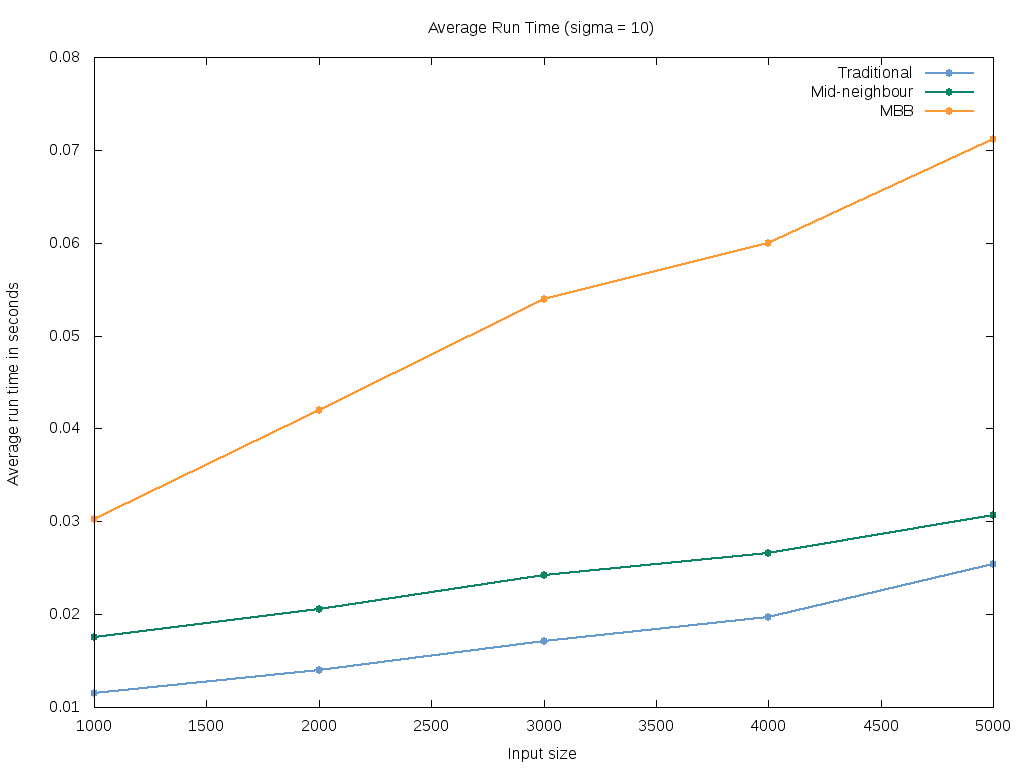
\includegraphics[scale=.3]{time_result}
        \end{figure}

    \end{itemize}
\end{frame}
\begin{frame}{Resultados}
    \begin{itemize}
        \item{Porcentagem do espaço de busca com calculo de custo:}
            \begin{figure}[h]
            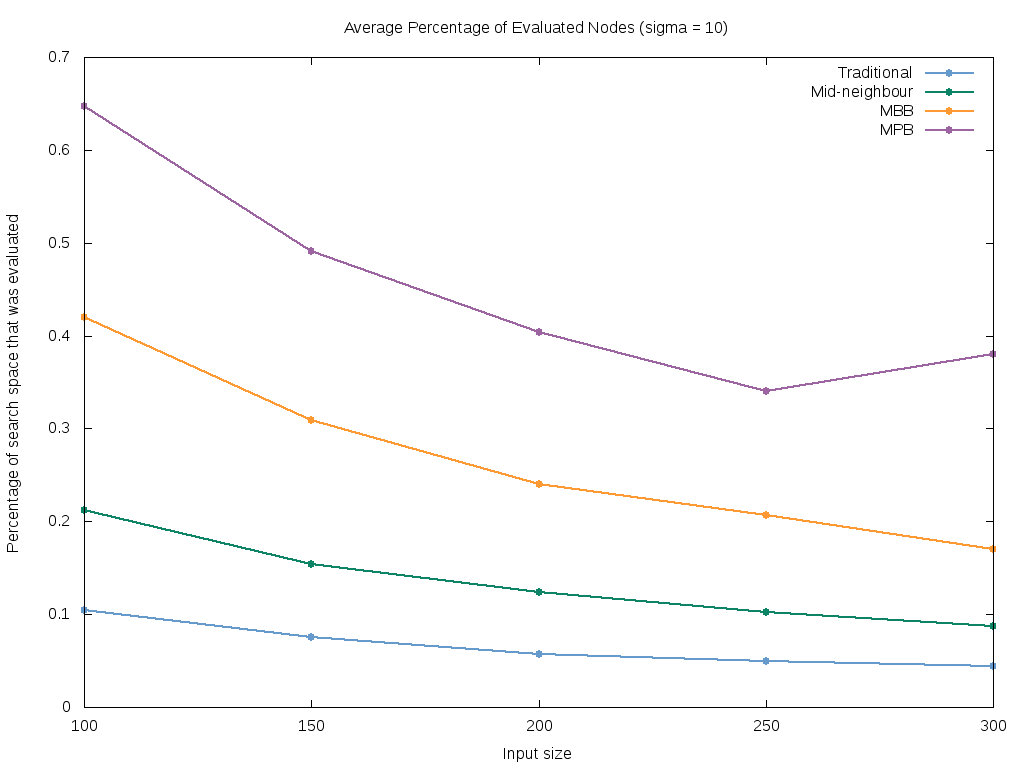
\includegraphics[scale=.3]{evaluations_result}
        \end{figure}
    \end{itemize}
\end{frame}
\begin{frame}{Resultados}
    \begin{itemize}
        \item{Corretude:}
            \begin{figure}[h]
            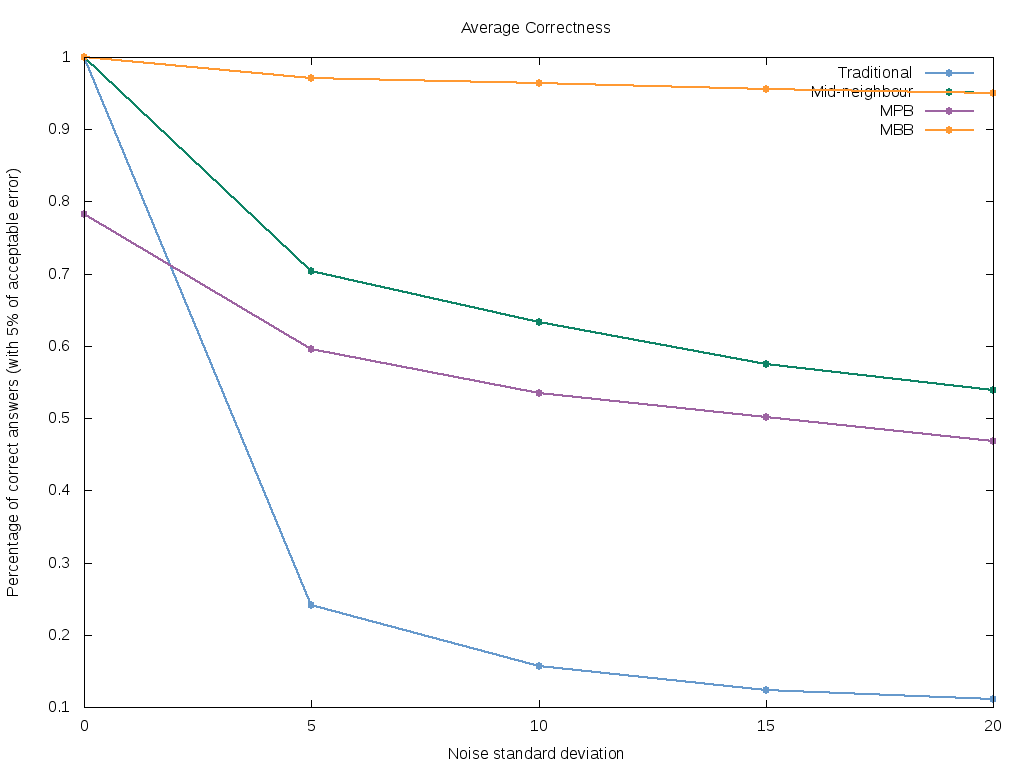
\includegraphics[scale=.3]{correctness_result}
        \end{figure}
    \end{itemize}
\end{frame}

\section{Referências}
\begin{frame}{Referências}
\begin{thebibliography}{9} \label{sec:referencias}
\addcontentsline{toc}{section}{Referências}
\bibitem{msreis thesis}
Reis, Marcelo S. ``Minimization of decomposable in U-shaped curves 
functions defined on poset chains–algorithms and applications." PhD
thesis, Institute of Mathematics and Statistics, University of São 
Paulo, Brazil, (2012).
\bibitem{ucs paper}
Reis, Marcelo S., Carlos E. Ferreira, and Junior Barrera. ``The U-curve
optimization problem: improvements on the original algorithm and time
complexity analysis." arXiv preprint arXiv:1407.6067, (2014). 
\bibitem{iubb}
Atashpaz-Gargari, Esmaeil, Ulisses M. Braga-Neto, and Edward R.
Dougherty. ``Improved branch-and-bound algorithm for U-curve 
optimization." 2013 IEEE International Workshop on Genomic Signal
Processing and Statistics (GENSIPS), (2013).
\end{thebibliography}
\end{frame}

\end{document}

